\section{Proof Architecture}\label{sec:proof-arch}
We now define relations that are proven using individual SNARKs, and that recursively combine into the final proof.

\subsection{Topology}

The proof pipeline consists of multiple circuit types.

\begin{instruction}
Teams should add footnotes to each circuit subsection below linking to the corresponding soundcalc entry for that circuit's parameters and security analysis.
\end{instruction}

Below we expose some aggregate information.

\begin{center}
\begin{tabular}{lccc}
\hline
\textbf{Circuit} & \textbf{Purpose} & Relations\\
\hline
\multicolumn{3}{l}{\emph{Inner segment circuits (leaf layer):}}\\
\quad\texttt{inner-step} & Segment trace & $\relation_{0,\step}$ \\
\quad\texttt{inner-keccak} & Keccak precompile & $\relation_{0,\keccak}$ \\
\quad\texttt{inner-poseidon} & Poseidon precompile & $\relation_{0,\poseidon}$ \\
\quad\texttt{inner-range} & Range checks & $\relation_{0,\range}$ \\
\hline
\texttt{segment}   & Segment proof       & $\relation_1$ \\
\texttt{convert}  & 1-to-1 normalization & $\relation_2$ \\
\texttt{combine}  & 2-to-1 merge     & $\relation_3$ \\
\texttt{embed}    & final proof      & $\relation_4$ \\
\hline
\end{tabular}
\end{center}


\begin{itemize}
  \item \emph{Inner segment circuits (leaf layer).} These four circuits jointly prove one segment; the \texttt{segment} circuit below verifies all four.
  \begin{itemize}[label=$\cdot$]
    \item \texttt{inner-step}: Proves the segment trace execution (with precompiles and range checks excluded).
    \item \texttt{inner-keccak}: Proves the Keccak precompile.
    \item \texttt{inner-poseidon}: Proves the Poseidon precompile.
    \item \texttt{inner-range}: Proves the range checks.
  \end{itemize}
	\item \texttt{segment}: Verifies the four inner proofs, effectively proving one segment
	\item \texttt{convert}: A 1-to-1 recursion circuit that verifies a single \texttt{segment} proof.
	\item \texttt{combine}: A recursive 2-to-1 circuit that verifies two child proofs, each of which may be either a \texttt{convert} or a \texttt{combine} proof.
	\item \texttt{embed}: The circuit that produces the final proof.
\end{itemize}


We visualize the recursion topology in Fig.~\ref{fig:topo}. Here,
$\pi^{\mathbf{0}}$ denotes the four inner proofs (one each for $\relation_{0,\step}$, $\relation_{0,\keccak}$, $\relation_{0,\poseidon}$, $\relation_{0,\range}$),
 $\pi^1$ are proofs of $\relation_1$ and thus the \texttt{segment} circuit. Similarly, $\pi^2$ proves the \texttt{convert} circuit, $\pi^3$ the \texttt{combine} circuit, and $\pi^4$ the \texttt{embed} circuit.

\begin{figure}
	\centering
	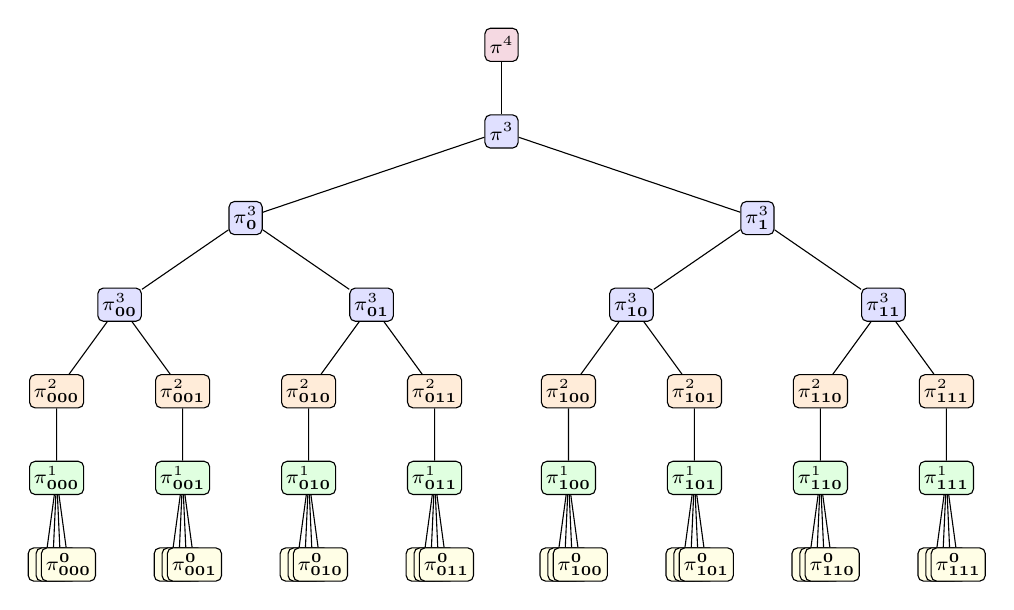
\begin{tikzpicture}[
		every node/.style={draw, rounded corners=2pt, minimum width=1.2em, minimum height=1.2em, inner sep=1.5pt, font=\scriptsize},
		embed/.style={fill=purple!15},
		combine/.style={fill=blue!12},
		convert/.style={fill=orange!15},
		riscv/.style={fill=green!12},
    base/.style={fill=yellow!10},
		level 1/.style={sibling distance=130mm},
		level 2/.style={sibling distance=65mm},
		level 3/.style={sibling distance=32mm},
		level 4/.style={sibling distance=16mm},
		level 5/.style={sibling distance=4mm},
		level 6/.style={sibling distance=1mm},
		level distance=11mm,
		edge from parent/.style={draw, thin},
		]
		\node [embed] {$\pi^{4}$}
		child { node [combine] {$\pi^{3}$}
			child {
				node [combine] {$\pi^{3}_{\bf 0}$}
				child {
					node [combine] {$\pi^{3}_{\bf 00}$}
					child { node [convert] {$\pi^{2}_{\bf 000}$}
						child { node [riscv] {$\pi^{1}_{\bf 000}$}
							child { node [base] {} }
							child { node [base] {} }
							child { node [base] {} }
							child { node [base] {$\pi^{\mathbf{0}}_{\bf 000}$} }
						}
					}
					child { node [convert] {$\pi^{2}_{\bf 001}$}
						child { node [riscv] {$\pi^{1}_{\bf 001}$}
							child { node [base] {} }
							child { node [base] {} }
							child { node [base] {} }
							child { node [base] {$\pi^{\mathbf{0}}_{\bf 001}$} }
						}
					}
				}
				child {
					node [combine] {$\pi^{3}_{\bf 01}$}
					child { node [convert] {$\pi^{2}_{\bf 010}$}
						child { node [riscv] {$\pi^{1}_{\bf 010}$}
							child { node [base] {} }
							child { node [base] {} }
							child { node [base] {} }
							child { node [base] {$\pi^{\mathbf{0}}_{\bf 010}$} }
						}
					}
					child { node [convert] {$\pi^{2}_{\bf 011}$}
						child { node [riscv] {$\pi^{1}_{\bf 011}$}
							child { node [base] {} }
							child { node [base] {} }
							child { node [base] {} }
							child { node [base] {$\pi^{\mathbf{0}}_{\bf 011}$} }
						}
					}
				}
			}
			child {
				node [combine] {$\pi^{3}_{\bf 1}$}
				child {
					node [combine] {$\pi^{3}_{\bf 10}$}
					child { node [convert] {$\pi^{2}_{\bf 100}$}
						child { node [riscv] {$\pi^{1}_{\bf 100}$}
							child { node [base] {} }
							child { node [base] {} }
							child { node [base] {} }
							child { node [base] {$\pi^{\mathbf{0}}_{\bf 100}$} }
						}
					}
					child { node [convert] {$\pi^{2}_{\bf 101}$}
						child { node [riscv] {$\pi^{1}_{\bf 101}$}
							child { node [base] {} }
							child { node [base] {} }
							child { node [base] {} }
							child { node [base] {$\pi^{\mathbf{0}}_{\bf 101}$} }
						}
					}
				}
				child {
					node [combine] {$\pi^{3}_{\bf 11}$}
					child { node [convert] {$\pi^{2}_{\bf 110}$}
						child { node [riscv] {$\pi^{1}_{\bf 110}$}
							child { node [base] {} }
							child { node [base] {} }
							child { node [base] {} }
							child { node [base] {$\pi^{\mathbf{0}}_{\bf 110}$} }
						}
					}
					child { node [convert] {$\pi^{2}_{\bf 111}$}
						child { node [riscv] {$\pi^{1}_{\bf 111}$}
							child { node [base] {} }
							child { node [base] {} }
							child { node [base] {} }
							child { node [base] {$\pi^{\mathbf{0}}_{\bf 111}$} }
						}
					}
				}
			}
		};
	\end{tikzpicture}
	\caption{\label{fig:topo} Recursion topology. Colors: \colorbox{yellow!10}{\texttt{inner}}, \colorbox{green!12}{\texttt{segment}}, \colorbox{orange!15}{\texttt{convert}}, \colorbox{blue!12}{\texttt{combine}}, \colorbox{purple!15}{\texttt{embed}}.}
\end{figure}

\subsection{\texttt{inner} circuits}

To optimize the proof size and prover time,
we introduce inner segment circuits that prove
the correctness of the segment trace, of precompiles,
and of range checks separately. As those
circuits share the same bus, we commit to the latter
to make the relations succinct.
These circuits are then recursively
combined  to prove the correctness of the full segment.

The first relation $\relation_{0,\step}$ chains
$N_{\text{seg}}$ consecutive valid steps
from $\hat{S}_{in}$ to $\hat{S}_{out}$,
with the bus committed in the public input.
The remaining three relations each assert correctness of
all entries of a given type in the bus
(Keccak, Poseidon, or range checks respectively),
again with the bus committed\footnote{Without loss
of generality we assume that the same commitment scheme is used for the bus.} in the public input.
\begin{equation}\label{eq:rel-inner-step}
  \scalebox{0.90}{$\displaystyle
    \relation_{0,\step} =\left(
    \left(\begin{array}{l}
      (\hat{S}_{in},\hat{S}_{out}, C_{\hat{\mathcal{B}}} );\;\\
      (\widehat{\BBB},\{\hat{S}_i\}_{1\leq i \leq {N_{\text{seg}}}+1},
      \{\pi^{\mathsf{mem}}_i\}_{1\leq i\leq N_{\text{seg}}})
    \end{array}\right)\;\Bigg|\quad
    \begin{array}{c}
      \hat{S}_1 = \hat{S}_{in}\\
      \hat{S}_{N_{\text{seg}}+1} = \hat{S}_{out}\\
      \bigwedge_{i=1}^{N_{\text{seg}}} \widehat{\pred{}}_{step,bus} (\hat{S}_i,\hat{S}_{i+1},\widehat{\BBB},\pi^{\mathsf{mem}}_i)=\mathrm{TRUE}\\
      C_{\hat{\mathcal{B}}} = \Com_{\mathsf{bus}}(\widehat{\BBB})
    \end{array}
   \right)
  $}
\end{equation}
where $\pi^{\mathsf{mem}}_i$ is the memory-opening witness for step~$i$: for a read step it is the Merkle authentication path $\pi$ required by $\widehat{\pred{}}_{\rea}$~\eqref{eq:op-mem-comm-read}; for a write step it is the pair $\pi^{\mathsf{mem}}_i = (\pi_{\writ}, v_{\mathsf{old}})$ required by $\widehat{\pred{}}_{\writ}$~\eqref{eq:op-mem-comm-write}; for all other steps it is unused.
The program code $\code$ is hard-wired into the \texttt{inner-step} circuit --- it appears in the fetch conjunct $\code[\pc_1]=op$ of each operation predicate via~\eqref{eq:phiop} --- so the \texttt{inner-step} verification key binds the proof to the fixed program.
\begin{equation}\label{eq:rel-inner-keccak}
  \relation_{0,\keccak} =\left(
   \left( C_{\hat{\mathcal{B}}} ;\;
  \widehat{\BBB} \right)\;\Bigg|\quad
  \begin{array}{c}
    \widehat{\pred{}}_{\keccak}(\widehat{\BBB})=\mathrm{TRUE}\\
    C_{\hat{\mathcal{B}}} = \Com_{\mathsf{bus}}(\widehat{\BBB})
  \end{array}
 \right)
\end{equation}
\begin{equation}\label{eq:rel-inner-poseidon}
  \relation_{0,\poseidon} =\left(
   \left( C_{\hat{\mathcal{B}}} ;\;
  \widehat{\BBB} \right)\;\Bigg|\quad
  \begin{array}{c}
    \widehat{\pred{}}_{\poseidon}(\widehat{\BBB})=\mathrm{TRUE}\\
    C_{\hat{\mathcal{B}}} = \Com_{\mathsf{bus}}(\widehat{\BBB})
  \end{array}
 \right)
\end{equation}
\begin{equation}\label{eq:rel-inner-range}
  \relation_{0,\range} =\left(
   \left( C_{\hat{\mathcal{B}}} ;\;
  \widehat{\BBB} \right)\;\Bigg|\quad
  \begin{array}{c}
    \widehat{\pred{}}_{\range}(\widehat{\BBB})=\mathrm{TRUE}\\
    C_{\hat{\mathcal{B}}} = \Com_{\mathsf{bus}}(\widehat{\BBB})
  \end{array}
 \right)
\end{equation}

The circuits are called, respectively,
\texttt{inner-step}, \texttt{inner-keccak}, \texttt{inner-poseidon}, and \texttt{inner-range}.
\begin{instruction}
Note that our writeup is a bit informal here, as we never formally defined $\Com$. Teams should do that, as the security analysis later will require a specific binding notion of $\Com$.
\end{instruction}

\subsection{ \texttt{segment} circuit}

The \texttt{segment} circuit recursively verifies the four inner proofs,
tying them together via a shared bus commitment $C_{\hat{\mathcal{B}}}$.
Let $\Pi_{0,j}=(\Pi_{0,j}.\mathsf{Prove}, \Pi_{0,j}.\mathsf{Verify})$
be the SNARK for $\relation_{0,j}$, where $j\in\{\step,\keccak,\poseidon,\range\}$.

\[
  \scalebox{0.90}{$\displaystyle
  \relation_1=\left\lbrace\begin{array}{c|c} (\hat{S}_{in},
   \hat{S}_{out});(C_{\hat{\mathcal{B}}},\pi_\step,\pi_\keccak,\pi_\poseidon,\pi_\range) &
    \begin{array}{c}
   \Pi_{0,\step}.\mathsf{Verify}((\hat{S}_{in},\, \hat{S}_{out},\, C_{\hat{\mathcal{B}}}), \pi_\step)=1\\
    \Pi_{0,\keccak}.\mathsf{Verify}( C_{\hat{\mathcal{B}}}, \pi_\keccak)=1\\
    \Pi_{0,\poseidon}.\mathsf{Verify}( C_{\hat{\mathcal{B}}}, \pi_\poseidon)=1\\
    \Pi_{0,\range}.\mathsf{Verify}( C_{\hat{\mathcal{B}}}, \pi_\range)=1
    \end{array}
  \end{array}\right\rbrace
  $}
\]


\subsection{\texttt{convert} circuit}

The \texttt{convert} circuit is a 1-to-1 recursion circuit that consumes a proof of $\relation_1$ and verifies it.  Its public
inputs are the boundary states and the segment size; its witness is the proof $\pi_1$. To formally define the relation,
let $\Pi_1=(\Pi_1.\mathsf{Prove}, \Pi_1.\mathsf{Verify})$ be the SNARK proving protocol for relation $\relation_1$.

$$\relation_2=\left\lbrace\begin{array}{c|c}
	((\hat{S}_0,\, \hat{S}_N,\, {N_{\text{seg}}});\; \pi_1) &
	\Pi_1.\mathsf{Verify}((\hat{S}_0,\, \hat{S}_N), \pi_1)=1
\end{array}\right\rbrace$$
Note that triples for which the last component is not ${N_{\text{seg}}}$ are never in $\relation_2$.

\subsection{\texttt{combine} circuit}

The \texttt{combine} circuit is a recursive 2-to-1 circuit that verifies two child proofs, each of which may be either a \texttt{convert} proof or another \texttt{combine} proof.
It checks three things:
\begin{itemize}
\item Each child proof is valid under $\Pi_2.\mathsf{Verify}$ if the child covers exactly one segment ($N_{child}=N_{\seg}$), or under $\Pi_3.\mathsf{Verify}$ if it covers at least two ($N_{child}\ge 2N_{\seg}$), where $\Pi_i=(\Pi_i.\mathsf{Prove}, \Pi_i.\mathsf{Verify})$ is the SNARK proving protocol for relation $\relation_i$.
\item The step counts satisfy $N_L + N_R = N$, with $N_L \geq N_{\seg}$, $N_R \geq N_{\seg}$, and both $N_L$, $N_R$ divisible by $N_{\seg}$, to ensure well-founded recursion and uniform segment structure.
\item State continuity: the witness $\hat{S}_N^L$ serves as both the final state of the left proof and the initial state of the right proof.
\end{itemize}
Since \texttt{combine} is self-recursive, repeated binary application naturally reduces any number of segment proofs into a single proof $\pi_3$ for the full execution.

For brevity, we write $\Vfy_i(\mathsf{x},\pi):=\Pi_i.\mathsf{Verify}(\mathsf{x},\pi)$.
\begin{equation}\label{eq:rel-combine-typed}
  \scalebox{0.85}{$\displaystyle
  \relation_3=\left\lbrace\begin{array}{c|c}
   ((\hat{S}_0^L,\, \hat{S}_N^R,\, N);\; (\pi^L,\, \pi^R,\, \hat{S}_N^L, N_L, N_R)) &
    \begin{array}{c}
   \bigl(N_L = N_{\seg} \wedge \Vfy_2((\hat{S}_0^L, \hat{S}_N^L, N_L),\, \pi^L)=1\bigr) \\
   {}\lor \bigl(N_L \geq 2N_{\seg} \wedge \Vfy_3((\hat{S}_0^L, \hat{S}_N^L, N_L),\, \pi^L)=1\bigr) \\
   \bigl(N_R = N_{\seg} \wedge \Vfy_2((\hat{S}_N^L, \hat{S}_N^R, N_R),\, \pi^R)=1\bigr) \\
   {}\lor \bigl(N_R \geq 2N_{\seg} \wedge \Vfy_3((\hat{S}_N^L, \hat{S}_N^R, N_R),\, \pi^R)=1\bigr) \\
   N_L + N_R = N \\
   N_{\seg} \mid N_L,\; N_{\seg} \mid N_R
    \end{array}
  \end{array}\right\rbrace
  $}
\end{equation}

where $\hat{S}_0^L$ and $\hat{S}_N^R$ are the public boundary states of the combined execution,
$\pi^L$ and $\pi^R$ are the two child proofs (each either a \texttt{convert} or \texttt{combine} proof), and $\hat{S}_N^L$ is the intermediate boundary state provided as witness.
The step count decides the child's type: a child covering exactly one segment
must carry a \texttt{convert} proof, a larger child a \texttt{combine} proof.
This typing is what entitles the extraction argument
(Lemma~\ref{lem:combine}) to treat every $\Vfy_2$-verified child as a
single-segment leaf: \emph{verification} of a proof for a statement outside a
relation's support is not excluded by knowledge soundness, so without the
typing the extractor could meet a verifying \texttt{convert} proof at a step
count it cannot use.  Completeness is unaffected --- an honest prover's
children have exactly these types.  (The bounds $N_L,N_R\ge N_{\seg}$ of the
untyped formulation are implied by the typing.)

\subsection{\texttt{embed} circuit}

The \texttt{embed} circuit produces the final proof, asserting correctness of the entire program execution
with public initial and final states. It assumes that
the total step count $T$ is known in advance to the verifier.
We fix $T$ as a publicly known system parameter satisfying $T \geq 2N_{\seg}$ and $N_{\seg} \mid T$
throughout, with $T \leq \mathsf{poly}(\lambda)$; these are standing assumptions on the system parameters and are not constraints
enforced by the circuit itself. The lower bound $T \geq 2N_{\seg}$ ensures that every execution
has at least two segments and hence admits a well-formed \texttt{combine} proof tree: a
single-segment execution ($T = N_{\seg}$) cannot be proven, because $\relation_3$ requires
$N_L + N_R = N$ with $N_L, N_R \geq N_{\seg}$, i.e.\ $N \geq 2N_{\seg}$.
Let $\Pi_3=(\Pi_3.\mathsf{Prove}, \Pi_3.\mathsf{Verify})$ be the SNARK proving protocol for relation $\relation_3$.

$$\relation_4=\left\lbrace\begin{array}{c|c}
	((\hat{S}_0,\, \hat{S}_T);\; \pi_3) &
	\Pi_3.\mathsf{Verify}((\hat{S}_0,\, \hat{S}_T,\,T),\, \pi_3)=1
\end{array}\right\rbrace$$

where $\hat{S}_0$ and $\hat{S}_T$ are the initial and final states of the entire program execution.

\begin{remark}[Divisibility requirement on $T$]
Since $\relation_3$ requires both child step counts to be divisible by $N_{\seg}$, every well-formed
\texttt{combine} proof tree has a total step count $N$ that is a multiple of $N_{\seg}$.
Consequently, the total step count $T$ passed to the \texttt{embed} circuit must satisfy
$N_{\seg} \mid T$.  The verifier checks this divisibility before invoking
$\Pi_3.\mathsf{Verify}$; proofs for step counts not divisible by $N_{\seg}$ are rejected outright.
\end{remark}

\begin{instruction}
  Teams should explain how the relations are proven using AIR / IOPs / poly-IOPs and the BCS transform. That is, teams should provide a direct reduction
from proving a relation to a low-degree test with
  FRI or another protocol. The reductions should contain links to the circuits submitted to soundcalc.
  The purpose of the section is to make explicit how the relations from the previous section are proven.
\end{instruction}

%----------------------------------------------------------------------
